\documentclass[columns=,boxcolor=white]{datart}

%\usepackage[top=1in,bottom=1in,left=1.2in,right=1.2in]{geometry}

%\usepackage{stmaryrd} % For those delicious brackets

% Title
\title{Big Data Problem with Machine Intelligence Stuff}
\date{}

\author[1]{Anders Roland Nielsen}
\author[1]{Andreas Berre Eriksen}
\author[1]{Kent Munthe Caspersen}
\author[1]{Mathias Melgaard Andersen}
\author[1]{Mikkel Alexander Madsen}
\author[1]{Sander Jespersen}

\affil[1]{Department of Computer Science, Aalborg University}

% CLEVEREF
%\crefname{tempDef}{Definition}{Definitions}
%\crefname{tempProof}{Proof}{Proofs}

%COMMANDS
%\usepackage{lmodern}

%HÜTTEL RULES
\providecommand{\condinfrule}[3]{\parbox{5.5cm}{\[ {\frac{#1}{#2}}{\qquad #3} \hfill \]}}
\providecommand{\infrule}[2]{\parbox{4.5cm}{\[\frac{#1}{#2}\hspace{.5cm}\]}}
\providecommand{\runa}[1]{\ensuremath{\tt{[#1]}}}
\providecommand{\single}[1]{\ensuremath{#1} \\}
\providecommand{\singlemat}[1]{\parbox{4.5cm}{\[#1\hspace{.5cm}\]}}
\providecommand{\bigrule}[2]{\genfrac{}{}{0pt}{0}{#1}{#2}}

% Gordon
% ----------------------------------------------------------------- %
% Horizontal brackets.                                              %
% ----------------------------------------------------------------- %

\newcommand{\hbra}{
%\hbox to .995       \columnwidth{\vrule width0.3mm height 1.8mm depth-0.3mm
\hbox to .995       \linewidth{\vrule width0.3mm height 1.8mm depth-0.3mm
                    \leaders\hrule height1.8mm depth-1.5mm\hfill
                    \vrule width0.3mm height 1.8mm depth-0.3mm}}
\newcommand{\hket}{
\hbox to .995 
%                    \columnwidth{\vrule width0.3mm height1.5mm
                    \linewidth{\vrule width0.3mm height1.5mm
                    \leaders\hrule height0.3mm\hfill
                    \vrule width0.3mm height1.5mm}}

% ----------------------------------------------------------------- %
% Typesetting definitions:                     output:              %
%                                                                   %
% \begin{defn}                                                      % 
% \Category{M,N}{terms}\\               M, N ::=      terms         %
% \entry{x}{variable}\\                   x             variable    % 
% \entry{M\ N}{application}\\             M N           application %
% \entry{\lambda x.\ M}{abstraction}      \x.M          abstraction %
% \end{defn}                                                        %
%                                                                   %
% This is a tabbing environment; the last entry should have no \\.  %
% ----------------------------------------------------------------- %

\makeatletter
  \newcommand{\addToLabel}[1]{%
    \protected@edef\@currentlabel{\@currentlabel#1}%
  }
\makeatother

\newcommand{\ratio}{.3}

\newenvironment{display}[1]{
  \pagebreak[2]% to prevent ugly broken displays
\begin{tabbing}
%\hspace{1.5em} \= \hspace{\ratio\columnwidth-1.5em} \= \hspace{1.5em} \= \hspace{1.5em} \= \kill
\hspace{1.5em} \= \hspace{\ratio\linewidth-1.5em} \= \hspace{1.5em} \= \hspace{1.5em} \= \kill
  {\bfseries#1}\\[-.7ex]
  \hbra\\[-.6ex]
  }{\\[-.7ex]\hket
  \end{tabbing}\vspace{-1.0ex}\normalsize}

\newcommand{\entry}[2]{\>$#1$\>\>#2}
\newcommand{\clause}[2]{$#1$\>\>#2}
\newcommand{\Category}[2]{\clause{#1::=}{#2}}
\newcommand{\simplecategory}[3]{\clause{#1::=#2}{#3}}
\newcommand{\subclause}[1]{\>\>\>#1}
\newcommand{\redrule}[3]{$#1$\>\>$#2$\>\>\>#3}

\newcommand{\labelledClause}[2]{%
  $#1$
  \>\>\>{\small #2}%
  \refstepcounter{rule}%
  \addToLabel{#2}%
}

\newcommand{\wlabelledClause}[2]{%
  $#1$
  \>\>\>\>{\small #2}%
  \refstepcounter{rule}%
  \addToLabel{#2}%
}


% \newcommand{\nodisplaybreak}[1]{ 
%   \noindent\begin{minipage}{\columnwidth}#1
%   \end{minipage}}

% \newcommand{\nofulldisplaybreak}[1]{ 
%   \iffull\begin{tabbing}\nodisplaybreak{#1}\end{tabbing}\else{#1}\fi}  \hbra\\[-.6ex]
%   }{\\[-.7ex]\hket
%   \end{tabbing}\vspace{-1.0ex}\normalsize}

% \newcommand{\entry}[2]{\>$#1$\>\>#2}
% \newcommand{\clause}[2]{$#1$\>\>#2}
% \newcommand{\Category}[2]{\clause{#1::=}{#2}}
% \newcommand{\simplecategory}[3]{\clause{#1::=#2}{#3}}
% \newcommand{\subclause}[1]{\>\>\>#1}
% \newcommand{\redrule}[3]{$#1$\>\>$#2$\>\>\>#3}




% document
\begin{document}
\maketitle

% ABSTRACT
\begin{abstract}
Here be dragons.
\end{abstract}

%%% Local Variables:
%%% mode: latex
%%% TeX-master: "main"
%%% End:


% CONTENT
\section{Introduction}\label{sec:intro}

Online multiplayer games have the possibility of generating a lot of data, this increases with the possible options for each individual player and the number of players. 
League of Legends (LoL), created by Riot games, was the most played online game in the beginning of 2015~\cite{LoLmostplayed}, mustering 27 million people playing it daily in the beginning of 2014~\cite{LoL27mill}. 

When playing, the players are divided into 2 competing teams (blue, purple) of 5 players each. In a classic match, each player will pick a champion(character) from a pool of 124 champions, each champion with 4 unique abilities. An ability is a magic spell, which does wildly different things, such as throwing a fireball at an opponent.
\\

\begin{wrapfigure}{r}{{0.5\textwidth}}
  \centering
    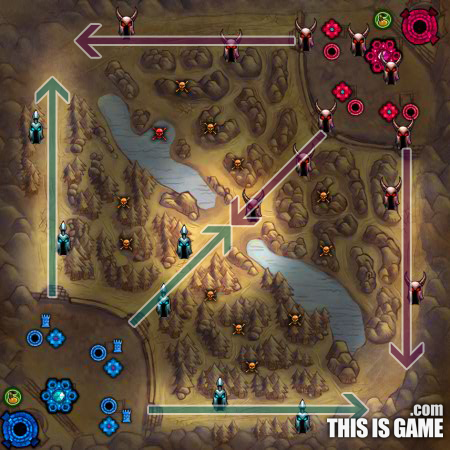
\includegraphics[width=0.5\textwidth]{Section1/lolmap.png}
  \caption{League of legends map}
\end{wrapfigure}\label{lolmap}
The map consists of three lanes(top, middle, bottom) as shown with arrows, connecting the two bases. In front of each lane in each base are two structures, an inhibitor and a turret defending the inhibtor. In the middle of the base is the nexus, which when destroyed ends the game, making the enemy team the winner. In each lane, the inhibitors spawn creeps(small monsters with low damage and health) which walks toward the opposing base on the lane it was spawned, the effect is that the two team's monsters meet in the middle, which is where the teams will fight, killing each others creeps. Furthermore, each lane has two extra turrets outside the base. A turret is a defensive structure fires at approaching enemies. When the inhibitor is destroyed, it makes the opposing team summon stronger minions. Lastly note that there is a "jungle", which consists of stronger monsters which award gold, and experience.
\\
Experience and money is earned through out the game for the individual players, when killing monsters or opposing players. The experience is used to improve the skills of the champion while money is spend purchasing items that will make the player stronger. This sums up the most important aspects of the game, and it is already quite clear how statespace the game hosts. This makes it extremely complex, and very interesting to analyse what one can do to improve ones gameplay. 
\\\\
The game combines strategy, individual player skill, communication and team play. It is a massive skill showcase, but how important is strategy? In this paper we will investigate how much of an advantage one can get by making good strategic decisions, based on a large dataset of matches played.


\subsection{Related Work}\label{sec:relatedwork}
K.\ Conley and D.\ Perry have trained a classifier to predict the winning team of a Dota 2 match~\cite{dota2article}, by only considering the heroes chosen at the beginning of the game. Dota 2 is game very similar to LOL.\@
Each feature used, represents the presence or absence of a particular hero on one of the teams.
When training on 18,000 matches they could correctly predict the outcome of 69.8 \% of the 5,669 matches in their test set.
With 50,000 training samples, they almost reached 70 \% correct predictions. Only matches between players of similiar skill levels were considered.

Konstantin Shvachko, et al.\, created Hadoop distributed file system (HDFS), to reliably handle very large data and to stream that data to user application at high bandwidth. They described the architecture and showed that it can successfully handle 25PB of Yahoo enterprice data~\cite{HDFS}.

Hadoop MapReduce and different variants have successfully been used for big data problems, by distributing the work load between many nodes in a cluster~\cite{DeanMapReduce}. 
Matei Zaharia, et al.\ have created Apache Spark and using this framework, the computation time is reduced if the data is being reused, in e.g.\ iterative machine learning or iterative data analysis tools~\cite{ApacheSpark}. 



%%% Local Variables:
%%% mode: latex
%%% TeX-master: "../main"
%%% End:
\subsection{Choosing features}\label{sec:choosingfeatures}
In the following, we aim to define the features $\phi_j(x)$ for each LoL match $x$, as described in \Cref{sec:phi}.
We define 5 different types of features and argue argue why each type is a good candidates for predicting the winning team.
The different types of features are each extracted by a mapping function, that maps a LoL match (in some cases with additional parameters) to a value. 
Before the feature mappings are defined, convenient notations are introduced that mathematically describes the concept of a game.
$C = \{1, 2, \dots, m\}$ is the set of all champions, where each champion is represented by an id. $m = 124$ for the patch version of LoL used in this project.
$P = \{p_1, p_2, \dots\}$ denotes the set of all players.
$T(x) = \{T_\text{blue}$, $T_\text{purple}\}$ is a set containing the two teams of match $x$, namely \emph{blue} and \emph{purple} respectively.
$T_i(x) = \{ (p_j, c_j) \in P \times C \mid c_j \text{ is controlled by } p_j \text{ on team } i  \text{ in match } x \}$.
$R = \{\text{unranked},\text{bronze},\text{silver},\text{gold},\text{platinum},\text{diamond},\text{master},\text{challenger},\}$ is the set of ranks.
$L = \{\text{top},\text{bottom},\text{mid},\text{jungle},\}$ is the set of lanes.
Some champions may be better than other champions. To capture the strength of individual champions, we will need a feature that represent the presence or absence of a particular champion on each team.
We define a feature $\phi_{\text{SINGLE}, t, c}(x)$, such that $\forall t \in T(x), \forall c \in C:$
\begin{equation}\label{eq:single}  
\phi_{\text{SINGLE}, t, c}(x) = 
\begin{cases} 
  1 & \text{if } (c, p) \in t \text{ for some } p \\
  0 & \text{otherwise} 
\end{cases}
\end{equation}



Some champions are considered damage dealers, they deal very high damage, but die easily. Other champions deal very little damage, but can be almost impossible to kill, these are considered tanks. These two types of champions are weak when alone, but when they team up, they can pose a serious threat. The tank can be used by the damage dealer as a living shield, allowing him to stay alive for much longer, thus deal more damage.
To capture the synergy between two champions on the same team, we will for each team need a feature that represents the presence or absence of every 2-combination of champions on that team. Therefore, we define a feature $\phi_{\text{PAIR},t, c_1, c_2}(x)$ such that $\forall t \in T(x), \forall c_1, c_2 \in C$ where $c_1 < c_2$:
\begin{equation}\label{eq:pair}
\phi_{\text{PAIR}, t, c_1, c_2}(x) =
\begin{cases}
  1 & \text{if } (c_1, p_1), (c_2, p_2) \in t \text{ for some }p_1, p_2\\
  0 & \text{otherwise}
\end{cases}
\end{equation}

We make the restriction $c_1 < c_2$, because we want to ignore permutations. This is because the two features $x_\text{PAIR}(t, c_1, c_2)$ and $x_\text{PAIR}(t, c_2, c_1)$ are the same, since they both capture that the two champions $c_1$ and $c_2$ are present on team $t$.

Some champions may have an advantage when fighting against a particular opponent.
For instance, a champion that is good at dodging ranged attacks is good against an enemy that only has ranged attacks.
We say that the better suited champion \emph{counters} the other.
To capture that one champion may counter another, we will for each champion on team $t$ need a feature that represents the presence or absence of every possible champion on the other team.
We define a feature $\phi_{\text{COUNTER},c_1,c_2}(x)$ such that $\forall c_1, c_2 \in C:$
\begin{equation}\label{eq:counter}
\phi_{\text{COUNTER},c_1,c_2}(x) = 
\begin{cases} 
1 & \text{if } (c_1, p_1) \in T_\text{blue}(x) \text{ and } (c_2, p_2) \in T_\text{purple}(x) \text{ for some } p_1, p_2 \\ 
0 & \text{otherwise} 
\end{cases}
\end{equation}

In this case, we do not have the restriction $c_1 < c_2$ and thus consider permutations instead of combinations.
To understand why, consider that $c_1$ counters $c_2$.
In this case, the feature $\phi_{\text{COUNTER},c_1,c_2}(x) = 1$ is favorable to the blue team, while $\phi_{\text{COUNTER},c_2,c_1}(x) = 1$ is favorable to the red team.
Note that in some game modes, $\phi_{\text{COUNTER},c_1,c_2}(x) = 1$, is allowed for $c_1 = c_2$. That is, the same champion may appear on both teams.
In that way we can capture if a champion can counter itself due to some asymmetries in the map layout.

In LoL, players can compete in ranked games, where they are placed in one of 7 tiers. Better players achieve higher tiers.
Before a match starts, we have access to data about the highest tier each player has achieved in a ranked game, which we will refer to as the rank of a player. We also know if a player has not competed in ranked games, in which case we say that he is unranked.
A player can achieve one of the ranks \textit{bronze}, \textit{silver}, \textit{gold}, \textit{platinum}, \textit{diamond}, \textit{master}, \textit{challenger} (mentioned in increasing order of skills required to achieve the rank).
We define a score function $\varphi : P \rightarrow \mathcal{N}$, where $\varphi(p) = 0$ if $p$ is unranked, or $1, 2, \dots, 7$ if $p$ has rank \textit{bronze}, \textit{silver}, $\dots$, \textit{challenger} respectively.
We define the rank of a team to be the average rank of all players on that team who is not unranked:
\begin{equation}\label{eq:eta}
\eta(t) = \frac{\sum\limits_{(p, c) \in t} \varphi(p)}{|\{(p, c) \in t \mid \varphi(p) > 0\}|}
\end{equation}
which we use to define a single feature
\begin{equation}\label{eq:bestrank}
\phi_\text{BEST-RANK}(x) = 
\begin{cases} 
  1 & \text{if } \eta(T_\text{blue}(x)) > \eta(T_\text{purple}(x))\\
  -1 & \text{if } \eta(T_\text{blue}(x)) < \eta(T_\text{blue}(x))\\
  0 & \text{otherwise} 
\end{cases}  
\end{equation}

The $\phi_\text{BEST-RANK}$ feature may have some shortcomings. The assumption that the rank of each player can be mapped to a score on a linear scale may not be entirely on spot.
Also, it may be easier to predict one team to be a winner, if the average rank of the two teams are considerably different. That is, if the players on one of the team have much greater ranks in average. The difference between the average rank of each team is not captured by the $\phi_\text{BEST-RANK}$ feature.
Therefore, another type of feature $\phi_{\text{PLAYER-RANK},p}(x)$ is introduced that captures the exact rank of each player.
$\forall(p, c) \in T_\text{blue}(x) \cup T_\text{purple}(x)$, we define a feature
\begin{equation}\label{eq:playerrank}
\phi_{\text{PLAYER-RANK},p}(x) = S(p)  
\end{equation}

In the early stage of a match, players tend to keep their champion in the same lane.
If a good player plays against a bad player in the same lane, the good player might get so strong, that the good player is able to carry the team to victory.
To define a new feature that considers the rank of players that play against each other in the same lane,
we first define a function that given a lane and team returns the rank of all players on the team that plays in that lane.
$\forall l \in L, \forall t \in T(x)$, we define
\begin{equation}\label{eq:xi}
  \xi(t,l) =
\begin{cases} 
  \text{none} & \text{if } \forall(c, p) \in t: c \text{ does not play in lane } l. \\
  r_1 & \text{if only } (c_1, p_1) \in t \text{ plays lane } l \text{ and } p_1 \text{ has rank } r_1 \text{.}\\
  (r_1, r_2) & \text{if only } (c_1, p_1), (c_2, p_2) \in t \text{ plays lane } l, \text{ where } p_1, p_2 \text{ has rank } r_1, r_2\\ 
&\text{respectively, and } p_1 \neq p_2.\\
  \text{many} & \text{otherwise}.
\end{cases}
\end{equation}

$\forall l \in L$, and for any $a,b$ that are possibles values in the range of $\xi$, we define the feature
\begin{equation}\label{eq:laneranks}
\phi_{\text{LANE-RANKS},l,a,b}(x) =
\begin{cases} 
  1 & \text{if } \xi(T_\text{BLUE}(x),l) = a, \xi(T_\text{PURPLE}(x),l) = b\\
  0 & \text{otherwise} 
\end{cases}  
\end{equation}

Some champions are better suited for a particular lane. For instance, mages tend to go mid as they generally loose both mana and health fast, and the path back to the base for regeneration is shortest from mid.
$\forall l \in L, \forall(p, c) \in T_\text{blue}(x) \cup T_\text{purple}(x)$, we define a feature
\begin{equation}\label{eq:championlane}
  \phi_{\text{CHAMPION-LANE},c,l}(x) =
\begin{cases} 
  1 & \text{if champion } c \text{ fought at lane } l)\\
  0 & \text{otherwise} 
\end{cases}
\end{equation}

\subsection{Feature sparsity}\label{sec:featuresparsity}
The size of $\phi_{\text{SINGLE}}$ is $|T(x)| \cdot |C| = 2 \cdot 124 = 248$. In each match, only $2 \cdot 5 = 10$ of those features appear. By appearance, we mean having a value of 1.\\
The size of $\phi_{\text{PAIR}}$ is $|T(x)| \cdot |C| \cdot (|C|-1) / 2 = 2 \cdot 124 \cdot 123 / 2 = 15252$. In each match, only $2 \cdot 5 \cdot 4 / 2 = 20$ of those features appear.\\
The size of $\phi_{\text{COUNTER}}$ is $|C|^2 = 124^2 = 15376$. In each match, only $5 \cdot 5 = 25$ of those features appear.\\
The size of $\phi_{\text{BEST-RANK}}$ is 3 by definition. In each match, only $1$ of those features appear.\\
The size of $\phi_{\text{PLAYER-RANK}}$ is $2 \cdot 5 \cdot 8 = 80$, since each of the $2$ teams have $5$ players, that each can have $1$ of $8$ ranks. In each match, only $10$ features appear, because each player has only $1$ rank.\\
The size of $\phi_{\text{LANE-RANKS}}$ is $|L| \cdot (2 + |R| + |R|^2)^2 = 21904$, because each lane contains either none, 1, 2, or many champions from each team.
In each match only $5$ of these features appear, as each of the lanes has exactly one combination of ranks of the players / champions playing against each other.
The size of $\phi_{\text{CHAMPION-LANE}}$ is $|T(x)| \cdot |C| \cdot |L| = 2 \cdot 124 \cdot 4 = 992$, because for each team, every champion can be in one of the 4 lanes. In each match, only $2 \cdot 5 \cdot 4 = 40$ features appear. 
These figures are presented in \Cref{tab:featuresparsity}, which also includes the number of features that appeared in $60.000$ LoL matches.

\begin{center}
\begin{table}[h]
\begin{tabular}{|l|ccc|}
\hline
Feature type                & Domain size & Appears in a single match & Appeared in 60,000 matches \\ \hline
$\phi_{\text{SINGLE}}$      & 248         & 10 & 248               \\ 
$\phi_{\text{PAIR}}$        & 15252       & 20 &                   \\ 
$\phi_{\text{COUNTER}}$     & 15376       & 25 & 15359             \\ 
$\phi_{\text{BEST-RANK}}$   & 3           & 1  & 3                 \\ 
$\phi_{\text{PLAYER-RANK}}$ & 80          & 10 & 80                \\ 
$\phi_{\text{LANE-RANKS}}$  & 21904       & 5  & 1834              \\ 
$\phi_{\text{CHAMPION-LANE}}$ & 992       & 40 & 992               \\ \hline
\end{tabular}
\caption{The sparsity of each type of feature}\label{tab:featuresparsity}
\end{table}
\end{center}

%%% Local Variables:
%%% mode: latex
%%% TeX-master: "../main"
%%% End:


\section{Representation of features}
\label{sec:representationoffeatures}
From the definition of features in section \ref{sec:choosingfeatures}, we can calculate that

\[|X_1| = |T| \cdot m \]

\[|X_2| = |T| \cdot \frac{m(m-1)}{2} \]

\[|X_3| = m^2  \]

where $m = |C|$ is the total number of champions in LoL.

With 123 total champions in LoL, we have that for each match:
$2 \cdot 5 = 10$ $X_1$ features are present out of 246 possible.
$2 \cdot (5 \cdot 4)/2 = 20$ $X_2$ features are present out of 15006 possible.
$5 \cdot 5 = 25$ $X_3$ features are present out of 15129 possible.
By present, we mean the features which value is 1.
It is clear that only a sparse number of features are present in each game. 

For optimizing the machine learning methods used, we will for each match only represent the features that are present in that game. 
Before applying a machine learning method, each of the features introduced in section \ref{sec:choosingfeatures} are assigned a unique ID.
For each match in the training data, the machine learning method is then given the IDs of the features present in that match.
We will now show how each feature in $X_1$, $X_2$, and $X_3$ is assigned a unique id:

\begin{center}
Every feature $x_1(t, c) \in X_1$ is given the ID:
\[ c + t \frac{|X_1|}{|T|} \]
\end{center}

It is easy to see that this assign unique IDs to all features in $X_1$.
Assigning unique IDs to features in $X_2$ is a bit more tricky since we are dealing with combinations and thus have the restriction $c_1 < c_2$.
If we enumerate all features $x_2(t, c_1, c_2) \in X_2$ for a single $t$ by $(c_1, c_2)$, we get the following enumeration:
\begin{align*}
(0, 1), (0, 2), (0, 3),& \dots, (0, m-1)\\
        (1, 2), (1, 3),& \dots, (1, m-1)\\
                        & \vdots    \\
                         &      (m-2, m-1)\\                   
\end{align*}
If using row and column indexes starting at $0$, we see that row $0$ contains $m-1$ elements, row $1$ contains $m-2$ elements, and so on.
That is, any row $i$ contains $m-1-i$ elements.
It is clear that the combination $(c_1, c_2)$ lies in row $c_1$ as element $c_2 - 1 - c_1$.
Thus, any combination $(c_1, c_2)$ is preceded by all elements in row $0$ through $c_1 - 1$, as well as $c_2 - 1 - c_1$ elements in its own row.
The number of elements in row $0$ through $c_1 - 1$ is an arithmetic series, and we can calculate the total number of elements
using the formula $n(a_0 + a_{n-1}/2$, where $n$ is the number of rows and $a_i$ is the number of elements in row $i$.
Since we have $m-1$ elements in row $0$ and $m - 1 - (c_1 - 1)$ elements in row $c_1 - 1$,
we get that $c_1(m-1 + m-1-(c_1-1))/2 = c_1(2m-1-c_1)/2$ elements are contained in the rows $0$ through $c_1 - 1$.
By adding the number of elements preceding $(c_1, c_2)$ in its own row, we get that $(c_1, c_2)$ is preceded by a total of
$c_1(2m-1-c_1)/2 + c_2-1-c_1 = c_1(2m-3-c_1)/2 + c_2-1$ elements.
We can now use the number of elements that precede $(c_1, c_2)$ as the ID for the feature $x_3(t, c_1, c_2)$. However, we must remember to add the offset $2m$, to not clash with the $x_t(c)$ features, and we must also add the offset $t \cdot m(m-1)/2$ since we for each $t \in T$ have $m(m-1)/2$ of the $x_3(t, c_1, c_2)$ features.
We finally get that:

\begin{center}
Every feature $x_2(t, c_1, c_2) \in X_2$, is given the ID:
\[ |X_1| + t \cdot \frac{|X_2|}{|T|} + \frac{c_1(2m-3-c_1)}{2} + c_2-1\]
\end{center}

Assigning an ID to the features in $X_3$ is simple since we are dealing with permutations. If we start enumerating all those features in the same way we did for the $X_2$ features, we will quickly see that the feature $x_3(c_1, c_2)$ appears as the $c_1m+c_2$'th element in the enumeration.
Now, we only need to add the correct offset of $|X_1| + |X_2| + |X_3|$, to get that:
\begin{center}
Every feature $x_3(c_1, c_2) \in X_4$ is given the ID:
\[|X_1| + |X_2| + c_1m+c_2\]
\end{center}

%%% Local Variables:
%%% mode: latex
%%% TeX-master: "../main"
%%% End:
\subsection{Logistic Regression}\label{sec:logistic}

To predict the outcome of a match, we use a linear classification model.
The model consists of a hypothesis function that is linear in the parameters.

\[ \hat{y} = w_0 + \sum_{j=1}^{M-1} w_j \phi_j(x) \]

Where $w_j$ represents the impact of of $\phi_j(x)$ on the hypothesis,
$w_0$ is the intercept and $\phi_j$ is a basis function that
performs a transformation on the input features. 

In order to classify the result of the hypothesis function into wins and losses. 
We use the so called logistic or sigmoid function.

\[ \sigma(\textbf{x}) = \frac{1}{1+e^{- \textbf{x}}} \]

The sigmoid function squashes the result of the hypothesis function into an inverval between one and zero.
This is appropriate because we never want a prediction less than zero or greater than one on a binary feature.
Furthermore the sigmoid function has a simple derivative that makes it easy to work with when using iterative methods.

\[ \sigma'(x) = \sigma(x) \times (1-\sigma(x)) \] 

\subsubsection{Cost Function}

In order to find the weights that produce the most accurate classification.
We minimise the squared error function.

\[ E_D = \sum_{n=1}^{N} \left(y_n - \textbf{w} \phi(\textbf{x}_n) \right)^2 \] 

\subsubsection{Regularisation}
To combat the problem of overfitting, we can use a method called L2-Regularisation.
In regularisation we penalise large weights, by adding the following term to the cost function.

\[ E_w = \lambda \sum_{j=1}^{M-1} w_j^2 \]

Where the regularisation constant $\lambda$ scales the penalty. 
The new cost function looks like this.

\[ E(\textbf{w})
  = E_D + E_w 
  = \sum_{n=1}^{N} \left(y_n - \textbf{w} \phi(\textbf{x}_n) \right)^2 + \lambda \sum_{j=1}^{M-1} w_j^2 \]

\begin{flushright}
\cite[online course]{courseraAI}
\end{flushright}

\subsubsection{Batch Gradient Descent}

Since we are using a large number of features, applying an analytic solution to find the weights quickly becomes impractical.
Therefore we use an iterative approach called batch gradient descent.

In gradient descent we iteratively update the weights by the partial derivative of the cost function with respect to the weight, multiplied by a learning rate $\eta$  
\[ w_j \leftarrow w_j - \eta \nabla_w E(\textbf{w}) \]

\subsubsection{Stochastic Gradient Descent}\label{sec:stochastic}

%When dealing with large data sets calculating the sum in the cost function becomes problematic.
 


% Non convergence of stochastic gradient descent





\begin{flushright}
\cite{Bishop2006}[p. ??]
\end{flushright}

% ###################################################################
%
%%\subsection{Logistic Regression}\label{sec:logistic}
%\subsection{Logistic Regression (old)}
%% logistic function
%
%For classification we use an activation function, whose purpose is to squash the result into the interval $(0,1)$.
%\[ f^{\overline{w}}(X_1, X_2, \dots X_n) = f(w_0 + w_1 \times X_1 + w_2 \times X_2 + \cdots + w_n \times X_n) \]
%
%\paragraph{Activation Functions}
%
%The most basic activation function is the so called step function defined as 
%\[ f(x) = \begin{cases}
%%	1 &\text{ if } f^{\overline{w}}(X_1,X_2, \text{ ... }, X_n) > 0 \\
%%	0 &\text{ if } f^{\overline{w}}(X_1,X_2, \text{ ... }, X_n) \leq 0 
%
%	1 &\text{ if } x \geq 0 \\
%	0 &\text{ if } x < 0 
%\end{cases}\]
%
%However the step function is not differentiable, and since this is a requirement for gradient descent we use another
%function called the sigmoid or logistic function.
%\[ f(x) = \frac{1}{1+e^{-x}} \]
%Unlike the previous activation function this function has a very simple derivative.
%
%\[ f'(x) = f(x) \times (1-f(x)) \]
%
%Which makes it easy to implement in a gradient descent algorithm.
%
%The cost function then becomes.
%\[ Error_E(\overline{w}) = \sum_{e \in E} \left(val(e,Y)-f\left(pval^{\overline{w}}(e,Y)\right)\right)^2 \]
%and the partial derivative becomes.
%\[ \frac{\partial \text{Error}_E(\overline{w})}{\partial w_i} 
%	= -2 \times \delta \times f'\left(\sum_i w_i \times val(e,X_i)\right) \times val(e,X_i) \]
%When using the sigmoid activation function the update step in gradient descent looks like this.
%\[ w_i := w_i + \eta \times \delta \times pval^{\overline{w}}(e,Y) \times \left(1 - pval^{\overline{w}}(e,Y)\right) \times val(e,X_i) \]
%
%Where $pval^{\overline{w}}(e,Y) = f(\sum_i w_i \times val(e,X_i))$.  
%
%
%\begin{flushright}
%\cite[p. 306-307]{AI2010}
%\end{flushright}
%
%
%\subsubsection{Regularisation}\label{sec:regular}
%To combat the problem of overfitting, we can use a method called regularisation.
%In regularisation we penalise large weights, by adding the following term to the cost function.
%
%% insert two pictures that show how regularization solves the overfitting problem.
%
%\[ \lambda \sum_{w_i \in \overline{w}} w_i^2 \]
%
%Where the regularisation constant $\lambda$ scales the penalty. 
%The new cost function looks like this.
%
%\[ Error_E(\overline{w}) = \sum_{e \in E} \left(val(e,Y) - pval^{\overline{w}}(e,Y)\right)^2 + \lambda \sum_{w_i \in \overline{w}} w_i^2 \]
%
%
%\begin{flushright}
%\cite[online course]{courseraAI}
%\end{flushright}

%\subsection{Large Datasets}
% Large datasets

% Stochastic regression












%%% Local Variables:
%%% mode: latex
%%% TeX-master: "../main"
%%% End:



%\section{Section 2}

%\section{Section 3}



\bibliography{Literature}

% APPENDIX
%\newpage
%\appendix

\end{document}

%%% Local Variables:
%%% mode: latex
%%% TeX-master: t
%%% End:
